\documentclass[12pt,a4paper]{article}
\usepackage[utf8]{inputenc}%Entrada estándar
\usepackage[T1]{fontenc}
\usepackage[spanish]{babel} %Para usar palabras reservadas en Español
\deactivatequoting
\usepackage{amsmath} %Matemáticas
\usepackage{amsfonts}%Fuentes
\usepackage{amssymb}%Símbolos
\usepackage{xcolor} %Para colores
\usepackage{fancyhdr} %Para las cabeceras y pie de página
\usepackage[hidelinks]{hyperref}
\usepackage{parskip}%Para espacios en párrafos
\usepackage{float}%Para figuras, tablas, entre otros.
\usepackage{listings}%Para listas
\usepackage{subfigure} % subfiguras
\usepackage{epstopdf} %para irlo transformando a PDF
\usepackage{setspace}%Espacios...
\usepackage{filecontents} %Para las referencias
\usepackage{cite} %Para la cita
\usepackage{geometry}%Márgenes
%\usepackage[left=2.54cm, right=2.94cm, top=2.54cm, bottom=2.54cm]{geometry}%Márgenes APA
\usepackage{blindtext} %Para listas
\usepackage{enumitem} %Para enumerar listas
\usepackage{array}
\usepackage{graphicx}
\usepackage{fontawesome}

%%%% DEFINICIÓN DE COLORES %%%%%
\definecolor{verde}{rgb}{0.13, 0.55, 0.13} 
\definecolor{azul}{rgb}{0.17, 0.48, 0.69}
\definecolor{rojo}{rgb}{0.8, 0.0, 0.0}
\definecolor{amarillo}{rgb}{1.0, 0.88, 0.21}
\definecolor{ambar}{rgb}{1.0, 0.49, 0.0}
\definecolor{rojo2}{rgb}{0.83, 0.0, 0.0}
%%%%%%%%%%%%%%%%%%%%%%%%%%%%%%%%%

%%        DIVERSOS USOS       %%%
\geometry{margin=2cm}

\setlength{\headheight}{100.2pt} %Espacio en la cabecera
 %Estilo de la cabecera
\fancyhf{} %Limpiar el estilo predefinido de cabecera
\lhead{
\includegraphics[scale=0.085]{escudoUNAM}} %Cabecera imagen izquierda
\rhead{
\includegraphics[scale=0.14]{escudoFI}} %Cabecera imagen derecha
%\fancyhead[RO,LE]{\thepage}
\fancyfoot[C]{\thepage}
%%%%%%%%%%%%%%%%%%%%%%%%%%%%%%%%%%%%%%%%%%%%%

%Para nuestra tabla de contenidos o índice%
\setcounter{secnumdepth}{5}
	
\setcounter{tocdepth}{4}
%%%%%%%%%%%%%%%%%%%%%%%%%%%%%%%%%%%%%%%%%%
\pagestyle{fancy}
\begin{document}
	\newgeometry{left=2cm, right=2cm, top=1cm, bottom=2cm}
	\begin{titlepage}
	\begin{center}
		{ 
			\begin{tabular}{p{0.7\textwidth} p{0.50\textwidth} }
				
\includegraphics[scale=0.18]{escudoUNAM} &  
\includegraphics[scale=0.29]{escudoFI}
			\end{tabular}
		}
		
		\textcolor{azul}{\rule{\linewidth}{0.8mm}}\\
		\vfill
		{\LARGE \textbf{Universidad Nacional Autónoma de México}}
		\vfill
		{\LARGE \textbf{Facultad de Ingeniería}}
		\vfill
		{\Large {División de Ingeniería Eléctrica}}
		\vfill
		{\Large {Departamento de Ingeniería en Computación}}
		\vfill
		{\huge {Estructuras de Datos y Algoritmos II}}
		\vfill
		{\LARGE {Grupo 9}}
		\vfill
		{\LARGE {Tista García, Edgar}}
		\vfill
		{\LARGE {Proyecto \#2: Programación Paralela\\}}
		\vspace{3mm}
		{\LARGE {Semestre 2021-1}}
		\vfill
		{\Large {Equipo 11\\}}
		\vfill
		{\Large {Integrantes:\\}}
		\vspace{3mm}
		{\Large {Díaz Hernández, Marcos Bryan\\}}
		\vspace{3mm}
		{\Large {Lara Aguilar, Christian Abraham\\}}
		\vfill
		{\LARGE {20 de Enero de 2021}}
	\end{center}
\end{titlepage} %Incluimos la carátula al principio
	\restoregeometry
	\newgeometry{left=2cm, right=2cm, top=4.5cm, bottom=2cm}
	\renewcommand{\footrulewidth}{1pt}
	%-----------------------------------------------------
	%Índice
	\tableofcontents
	\vfill
	\clearpage
	%-----------------------------------------------------
	
	\section{Introducción}
		Los fractales son estructuras geométricas que se caracterizan por estar compuestas por sí mismas en distintas proporciones, uno de estos entes matemáticos el cual consideramos el más interesantes de este tipo el el fractal de Mandelbrot o también conocido como set - Mandelbrot.
		
		El fractal de Mandelbrot es conocido por la complejidad que se ve intrínseca en este debido a que su representación se encuentra dentro de los números imaginarios y por la dificultad que se encuentra en la misma irregularidad, ya que la representación matemática de estos no es una tarea sencilla de poder llevar a cabo. Sin embargo, gracias al avance tecnológico es posible delegar tareas a los procesadores de nuestras computadoras, ya que cuentan con el poder de procesamiento necesario. 
		
		Debido a lo anterior y con el objetivo del proyecto nos enfocamos en encontrar un algoritmo que pudiera llevar a cabo la representación gráfica de este fractal, por medio de las operaciones con los números complejos es posible el llevar a cabo un algoritmo que verifica la convergencia de un conjunto de píxeles, dentro de un radio de convergencia y en base a esto poder asignarle un color al pixel, de forma que al llevar a cabo esto dentro un conjunto iterativo es posible es crear un gráfico que representa el fractal de mandelbrot.
		
		Pero debido a lo anterior y a la naturaleza de ser un fractal se pueden realizar acercamientos dentro de este ente geométrico, de tal modo que es posible ver la estructura base del fractal n veces en distintos tamaños, componiendose a sí misma, este zoom es posible realizarlo por medio del paralelismo en la programación.
		
		El paralelismo permite que se pueda realizar el zoom al mismo momento en que se van creando cada una de las imágenes que manifiestan este proceso en secuencia, y por medio de hilos o procesadores es posible disponer de la creación de esta secuencia.
		
		\subsection{Objetivo general}
			Que el alumno ponga en práctica los conceptos de la programación paralela a través de la implementación de un algoritmo paralelo, así mismo desarrolle su capacidad para responder preguntas acerca de un concepto analizado a profundidad
		\subsection{Objetivo del equipo}
			Aplicar la teoría de programación concurrente en Java para poder crear la representación del fractal conocido más famoso de todos, el conjunto de Mandelbrot. Así mismo, el comprobar cómo cambiando los parámetros de ciertos datos van formando y variando a este conjunto.
	
	\section{Antecedentes}
		El fractal de Mandelbrot es un conjunto de puntos dentro del plano imaginario, que se origina a partir del análisis de los elementos naturales más simples como lo es una coliflor, debido a que ésta cuenta con la característica especial de que al ser cortada de la forma que sea, se obtiene una versión pequeña de la misma; un fractal. Por ello es necesario el comenzar con la definición de lo que es un fractal: \textit{objeto geométrico en el que una misma estructura, fragmentada o aparentemente irregular, se repite a diferentes escalas y tamaños}
		
		\begin{figure}[h]
			\centering
			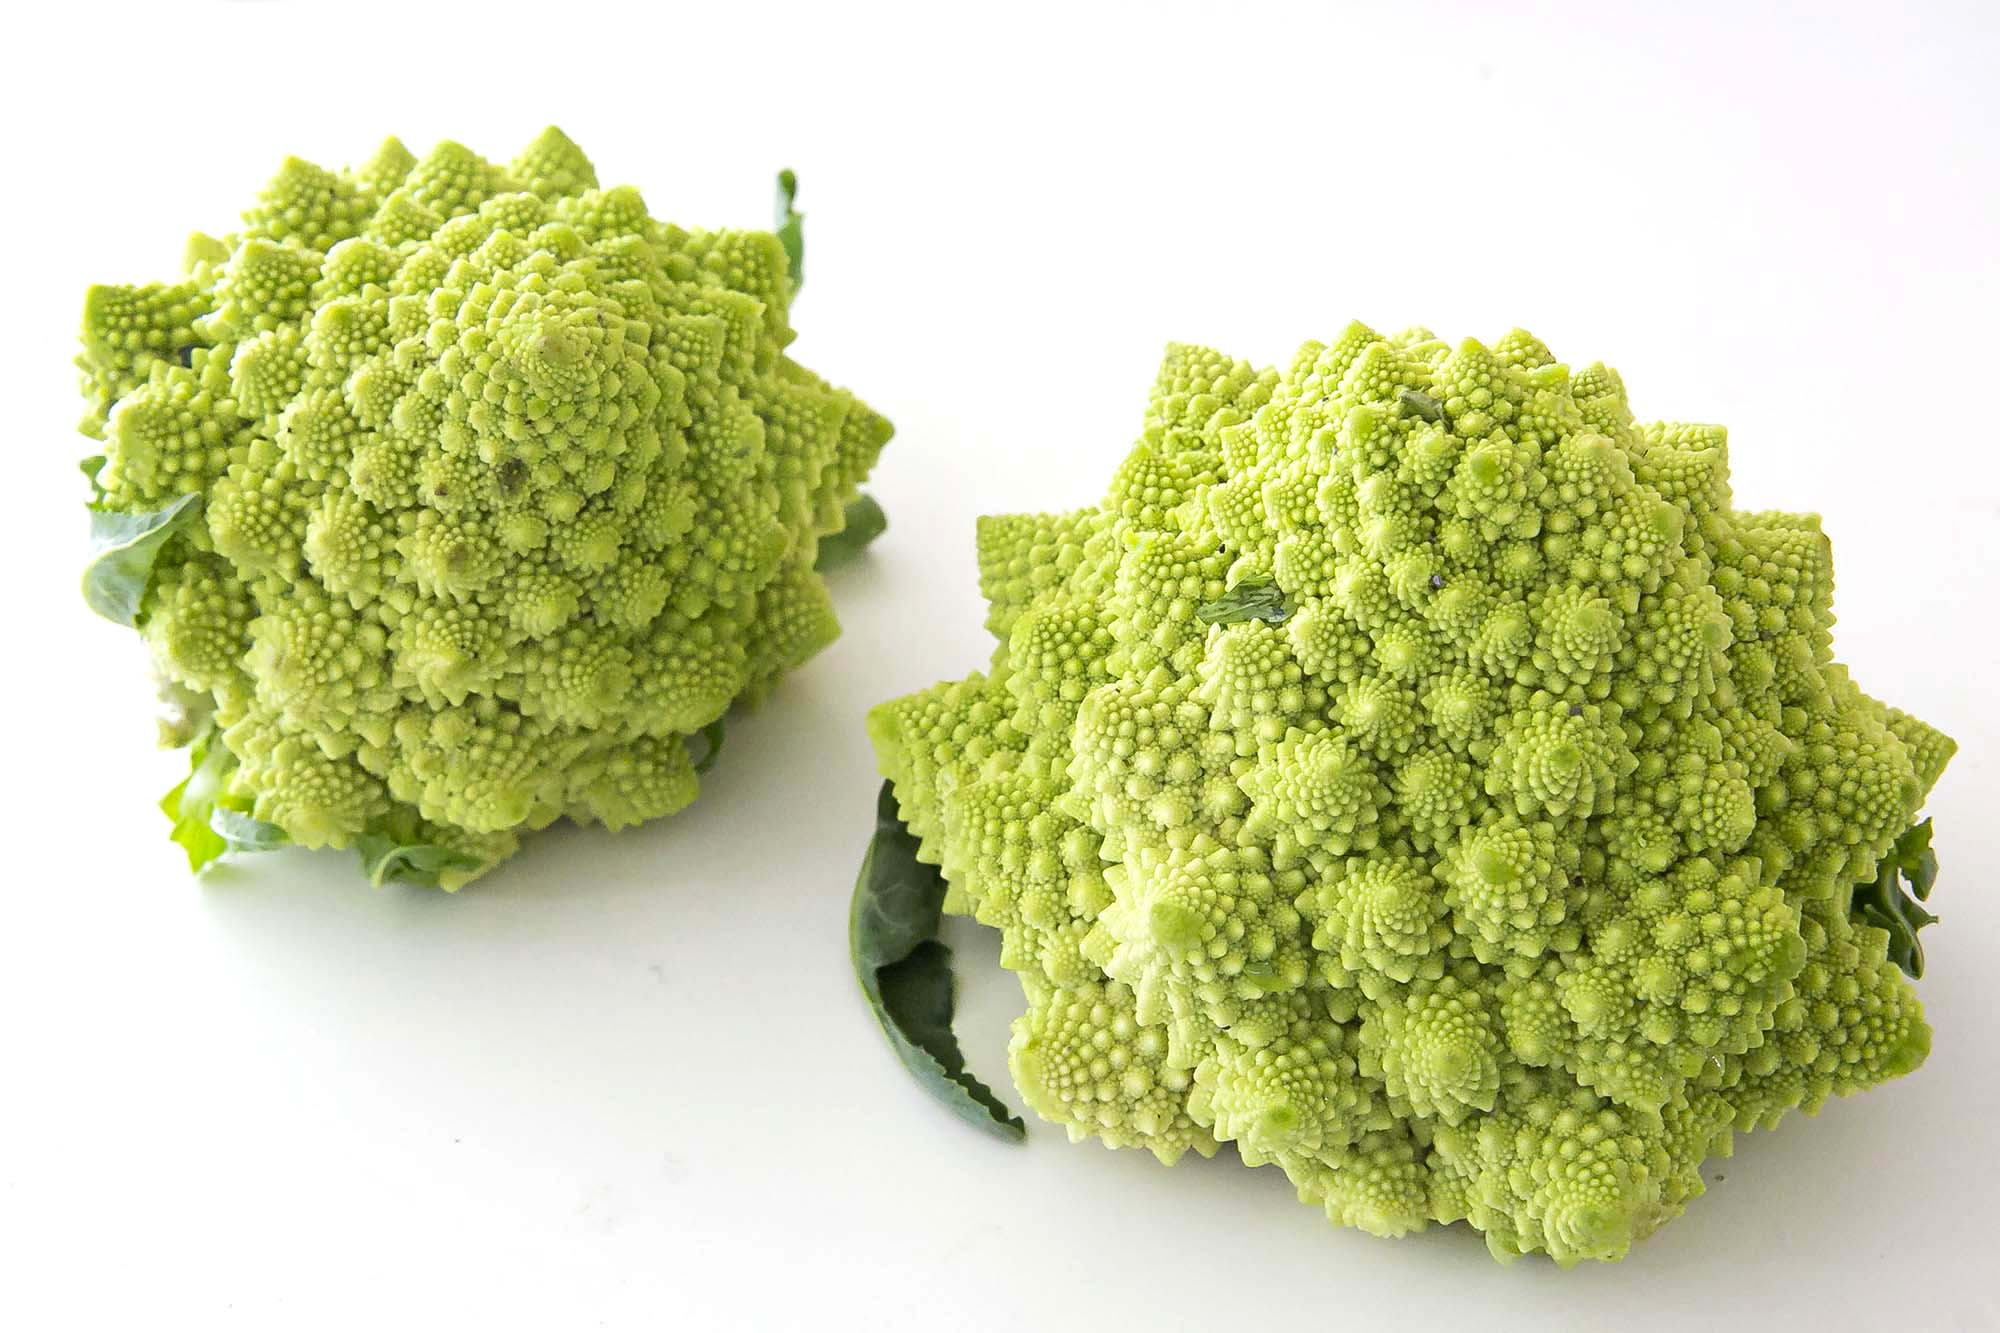
\includegraphics[scale=0.11]{romanesco}
			\caption{Coliflor romanesco}
		\end{figure}
				
		Continuando con la definición del fractal de Mandelbrot, este se crea dentro de un plano complejo, por lo que para poder comprender cómo se emplea este en la implementación del algoritmo es necesario explicarlo. El plano de Argand, o plano complejo, se caracteriza por tener dos ejes perpendiculares, donde el vertical corresponde al eje imaginario y el horizontal  al eje real, de tal forma que los números complejos están compuestos de una parte real y una parte imaginaria. La parte imaginaria que compone al número complejo, axiomáticamente se define como $\sqrt{-1} = i$, por lo cual, si se tiene, por ejemplo, al número $z = 4 + \sqrt{-16}$ se puede reescribir como $z = 4 + \sqrt{(16)(-1)}$ que es igual a $z = 4 + (\sqrt{(16)}\sqrt{-1})$ que sería $z = 4 + 4i$.
				
		\begin{figure}[h]
			\centering
			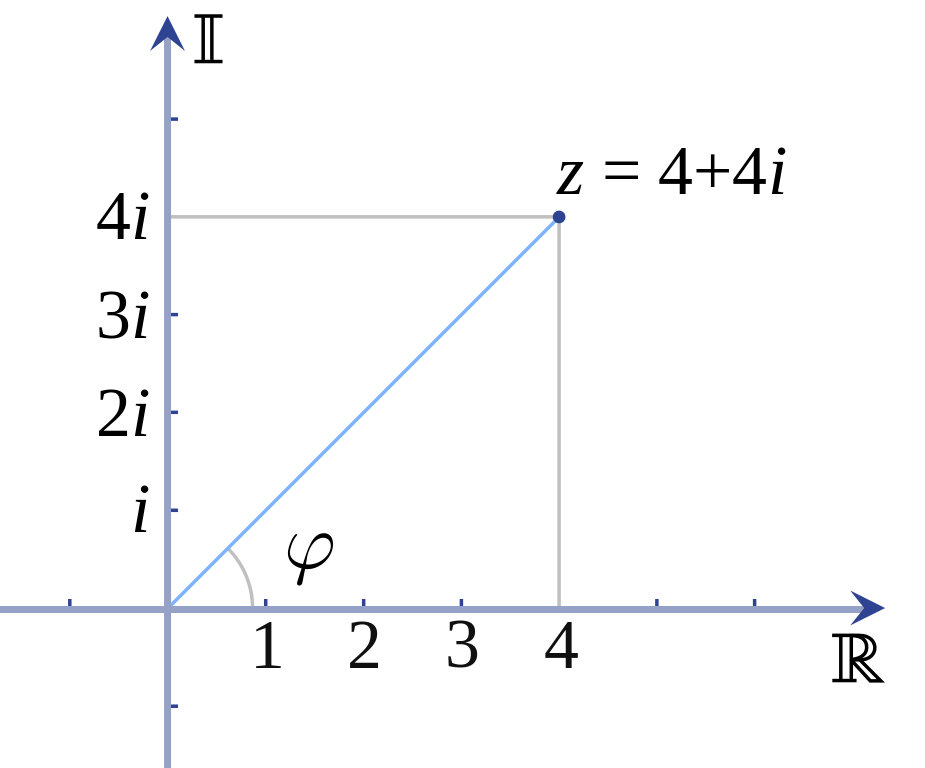
\includegraphics[scale=0.15]{planocomplejo}
			\caption{El plano complejo}
		\end{figure}
		
		Es posible realizar las operaciones más simples como la multiplicación, la suma, la resta y la división en este plano, respetando los tipos de datos, es decir que los reales se simplifican con los reales y los imaginarios de igual forma con sus correspondientes. Cada uno de los números complejos se representan, o se pueden representar, por medio de tres formas: polar, matricial y vectorial.\\
		En base a lo que se expondrá en la descripción del algoritmo, se deberá considerar lo siguiente, que la expresión: $\mathbf{f(z) = z^2 + c}$, es una operación donde $c = a + bi$ es un número complejo, donde $a$ representa la parte real, y $bi$ la parte imaginaria. Por medio de las iteraciones, este valor comienza recorrer el plano de imaginario, que para aplicaciones prácticas se limita a una región determinada, y a un radio que permita el determinar la convergencia.
				
		Uno de los elementos más complejos dentro de la comprobación del fractal de Mandelbrot, fue el demostrar su composición, tanto de forma analítica como practica. Dentro de la analítica no bastaba con únicamente decir que estaba compuesto por sí mismo en diferentes dimensiones y que contaba con cierto grado de fracturación. Era necesaria la demostración matemática que se explica dentro de la descripción del algoritmo.  
		
	\section{Descripción del algoritmo, estructura paralela seleccionada}
		El conjunto de Mandelbrot se compone por la siguiente regla iterativa:
 		\begin{center}
			$z_{n+1} = z_{n}^2 + c$
		\end{center}
		
		Con  $Z_{0} = 0$ y siendo $c$ todos los puntos del plano complejo. Al ir evaluando puntos del plano complejo, notaremos que existen dos situaciones en la que nos encontremos.\\
		Si, por ejemplo, tomamos a $c = 1$, veremos los primeros términos siguientes:
		\begin{center}
			$Z_{0} = 0$\\
			$Z_{1} = 0^2 + 1 = 1$\\
			$Z_{2} = 1^2 + 1 = 2$\\
			$Z_{3} = 2^2 + 1 = 5$\\
			$Z_{4} = 5^2 + 1 = 26$\\
			$Z_{5} = 26^2 + 1 = 677$\\
			$Z_{6}= 677^2 + 1 = 458330$\\
		\end{center}
	
		Como se puede apreciar, con $c = 1$, nuestra expresión crecería hasta el infinito.\\
		Por otro lado, si consideramos el caso de $c = -1$, tendremos los siguientes primeros términos:
		\begin{center}
			$Z_{0} = 0$\\
			$Z_{1} = 0^2 - 1 = -1$\\
			$Z_{2} = (-1)^2 - 1 = 0$\\
			$Z_{3} = 0^2 - 1 = -1$\\
			$Z_{4} = (-1)^2 - 1 = 0$\\
			$Z_{5} = 0^2 - 1 = -1$\\
			$Z_{6}= (-1)^2 - 1 = 0$\\
		\end{center}
		Donde podremos notar que el punto $c = 1$ del plano complejo, jamás alcanzará una magnitud mayor que $1$.

		En general, \textbf{el conjunto de Mandelbrot} se define como \textit{el conjunto de todos los puntos \textbf{c} del plano complejo para los que la iteración definida $\mathbf{z_{n+1} = z_{n}^2 + c}$ no diverge}. De acuerdo a esta definición, podemos asegurar que el caso de $c = 1$ no pertenece a este conjunto, pues la iteración en la expresión con este valor tiende al infinito, mientras que con $c = -1$ aseguramos que estarán acotados los resultados de la expresión iterativa, es decir, que no divergen, por lo tanto, \textbf{pertenecen al conjunto de Mandelbrot}.
		
		Para obtener más puntos del plano complejo se podrían calcular una inmensidad de valores para obtener sólo aquellos que sí pertenecen a este conjunto, una tarea imposible de realizar a mano, pero que con ayuda de computadoras puede ser posible mediante una representación gráfica.
		
		Cabe mencionar que matemáticamente se sabe que todos los puntos para los que $|c| > 2$ son puntos que divergen, por lo que, por la misma razón, cualquier $c$ para la que en algún punto de la iteración $|Z_{n}| > 2$ también serán puntos que diverjan y necesariamente no son parte del conjunto de Mandelbrot.
		
		Así pues, el evaluar un punto exacto en esta expresión iterativa puede llevarnos a estancarnos en un bucle infinito en el cual los valores siempre permanecerán en nuestro \textbf{radio de convergencia} (menor o igual a 2), lo cual sería contraproducente pues se calcularían indefinidamente los mismos valores obtenidos. Para resolver este inconveniente es que se utiliza una variable llamada \textbf{número de iteraciones}, mediante la cual podremos limitar el número de veces que se calculará la expresión en el plano complejo para un valor $c$ dado. Además de poder ocupar el número de iteraciones para no sobrecargar de trabajo innecesario a la computadora, se puede utilizar este mismo número para poder saber a partir de qué iteración nuestro valor en el plano complejo se sale de nuestro radio de convergencia, para así, crear una especie de \textbf{“mapa de calor”} en el que la gradiente de color represente el número de iteraciones.
	
		
	\section{Paralelización del algoritmo}	
		\subsection{Tipo de paralelismo}
			El algoritmo utilizado para este proyecto está pensado en ser paralelo, pero debido a la  \textit{naturaleza intrínseca} del lenguaje de programación \textbf{Java}, éste sólo puede ser expresado de forma serial o concurrente. Por lo cual, la versión presentada en este proyecto es la versión concurrente del conjunto de Mandelbrot.
			
			Si existiese la posibilidad de que sea totalmente paralelo, se seguiría la \textbf{Paralelización geométrica}, debido a que la gran carga y la diferencia entre su versión serial está en la parte de calcular y pintar cada píxel para crear una imagen, es decir, al momento de los cálculos para crear la imagen y pintarla, no se requiere de conexión con otros hilos de una manera que dependa de obtener información de ellos, por lo que el programa se divide de una manera simétrica en la cual cada proceso es responsable de una región espacial de los datos, en este caso de las imágenes creadas.
			
		\subsection{Métricas de desempeño}
			\subsubsection{Tiempos de procesamiento y comunicación}
				Se obtuvieron los siguientes tiempos para diferentes hilos y la misma carga de trabajo para cada hilo (8 imágenes en total):\\
				
					\begin{table}[htbp]
						\centering
						\begin{tabular}{c|c|c}
							Hilos & Imágenes & Tiempo(ms) \\ \hline
							1     & 8        & 33199  \\
							2     & 4        & 18139  \\
							4     & 2        & 10444  \\
							8     & 1        & 9677  
						\end{tabular}
					\end{table}
				
			\subsubsection{Speedup}
				El Speedup relaciona el tiempo de ejecución de un solo procesador con el tiempo de ejecución en varios procesadores, así, a partir de la expresión
				\begin{center}
					$S(n) = \dfrac{T(1)}{T(n)}$
				\end{center}
				se obtuvieron los siguientes resultados:
				\begin{center}
					$S(2) = \dfrac{33199}{18139} =  1.8302$\\
					 \vspace{.8cm}
					$S(4) = \dfrac{33199}{10444} = 3.1787$\\
				 	 \vspace{.8cm}
					$S(8) = \dfrac{33199}{9677} = 3.4307$
				\end{center}
							
			\subsubsection{Eficiencia}
				La medida de eficiencia se asocia a la idea que $n$ procesadores deben hacer el trabajo en una fracción $\dfrac{1}{n}$ del tiempo que le lleva a un solo procesador. Este valor refleja el aprovechamiento de los recursos de hardware del sistema, por lo que siempre será un valor menor a $1$\\
				Utilizando la expresión
				\begin{center}
					$E(n) = \dfrac{T(1)}{nT(n)} = \dfrac{S(n)}{n}$
				\end{center}
				se obtuvieron los siguientes resultados:
				\begin{center}
					$E(2) = 0.9151$\\
					$E(4) = 0.7946$\\
					$E(8) = 0.4288$
				\end{center}
							
			\subsubsection{Fracción serial}
				Esta métrica de desempeño relaciona el Speedup y la eficiencia, con el propósito de tomar en cuenta otros factores además del tiempo.\\
				Su expresión está dada por
				\begin{center}
					$f = \dfrac{\dfrac{1}{S} - \dfrac{1}{n}}{1 - \dfrac{1}{n}}$
				\end{center}
				Los resultados obtenidos para 2, 4 y 8 hilos se muestran a continuación:
				\begin{table}[htbp]
					\begin{tabular}{l|l|l}
						$f(2) = \dfrac{\dfrac{1}{3.4307}-\dfrac{1}{2}}{1-\dfrac{1}{2}} = 0.19026$ & $f(4) = \dfrac{\dfrac{1}{3.4307}-\dfrac{1}{4}}{1-\dfrac{1}{4}} = 0.08612$ & $f(8) = \dfrac{\dfrac{1}{3.4307}-\dfrac{1}{8}}{1-\dfrac{1}{8}} = 0.09277$
					\end{tabular}
				\end{table}
						
		\subsection{Formas de comunicación}
		\begin{description}
			\item[\faCheckSquareO  Local] Se comunica de manera local, pues desde el \textit{main} se comunica con los otros hilos
			\item[\faCheckSquareO  No estructurado] La forma en la que se comunican los hilos no está estructurada 
			\item[\faCheckSquareO  Estática] Su forma de comunicación se define antes de la ejecución del programa
			\item[\faCheckSquareO  Asíncrona] No se requiere de algún tipo de semáforo o variable especial para el acceso a los datos
		\end{description}
		
		\subsection{Granularidad}
		De acuerdo a la implementación paralela del programa se puede observar que tiene una granularidad gruesa, esto se debe a que cada hilo implementado y/o creado no necesita una gran sincronización entre los hilos creados, esto se puede apreciar dentro de la clase main del código pues con la ayuda de un ciclo for cada hilo se va inicializando uno por uno y cada hilo se encarga de crear un número determinado de imágenes a partir de ciertos datos, los cuales si bien varían, no son enviados precisamente entre los hilos para la creación de las imágenes.
	
	\section{Implementación del algoritmo paralelo}
		\subsection{Java(bibliotecas concurrentes y paralelas)}
			\textbf{import java.awt.image.BufferedImage}\\
			La clase permite crear un buffer para poder crear el espacio de una imagen, en este caso el algoritmo crea varias imágenes debido a la posibilidad de establecer un zoom (que en realidad vuelve a crear la imagen con una escala mayor) a través de la creación del fractal. El método constructor permite colocar las dimensiones de la imagen o imágenes que se van a crear, además de poder colocar el tipo de imagen, que en este caso es una imagen del tipo RGB.
			
			\begin{figure}[h]
				\centering
				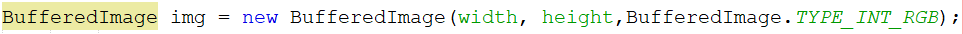
\includegraphics[width=\linewidth]{bufferedimage}
				\caption{Objeto de tipo BufferedImage}
			\end{figure}
			
			El método \textbf{setRGB}, permite asignarle un color al pixel en el que se esté trabajando durante la iteración del algoritmo, para ello se necesitan las coordenadas y  color que se le va a asignar.
			
			\begin{figure}[h]
				\centering
				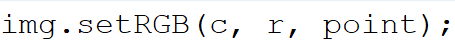
\includegraphics[scale=.5]{setrgb}
				\caption{Método setRGB}
			\end{figure}
			
			
			\textbf{import java.io.File;}\\
			La clase permite el manejo de los archivos, por medio de esta se puede transmitir la información para la escritura de la imagen, y poder crear las imágenes que cada uno de los hilos terminará realizando, ya que el algoritmo utiliza un arreglo de hilos para poder asignarles una cantidad de imágenes que representen los zoom de fractal. 
			\begin{figure}[h]
				\centering
				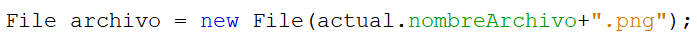
\includegraphics[scale=0.7]{file}
				\caption{Objeto de tipo File}
			\end{figure}
						
			\textbf{import javax.imageio.ImageIO;}\\
			La clase permite la escritura en imágenes, por medio del método write, al cual es necesario el enviarle un objeto de BufferedImage y un File. Se debe agregar entre un \textit{try-catch} debido a que arroja una excepción en caso de haber un error al escribir en el archivo o leerlo:
			\begin{figure}[H]
				\centering
				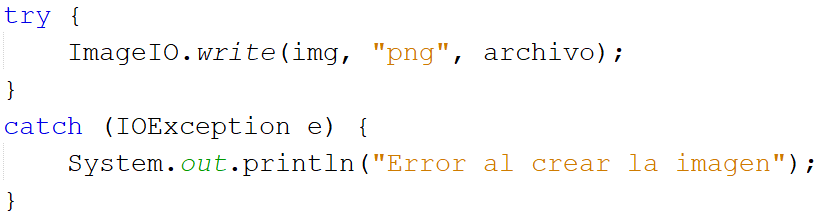
\includegraphics[scale=0.5]{imageio}
				\caption{Clase ImageIO, método write}
			\end{figure}
			
			Donde el Buffered utiliza la interfaz RenderedImage, para poder crear la imagen por medio de la asignación de los colores a los pixeles, y se utiliza el objeto File para poder crear la imagen, y por medio del nombre crear el tipo de imagen que se especifica.\\
			Una vez conocidas estas clases y métodos, se procede a explicar el programa:\\
			Existen cuatro clases para este programa, las cuales son \textbf{Main, Colores, Parametros y Renderizado}, cada una de ellas se especializa en diferentes tareas, pero sólo la clase \textbf{Renderizado} implementa a \textbf{Runnable} para la creación de los hilos y su uso mediante el método \textit{run}.\\
			Desde la clase \textbf{Main} es donde se elige el número de hilos a usar, así como el número de imágenes que creará cada uno de estos hilos, el nombre de los archivos así como su contador (para no sobrescribir el mismo archivo, claramente), además, se escoge la resolución inicial, la resolución tras cada imagen nueva creada, el centro de la imagen y el número de iteraciones máximas a calcular. Una vez elegidos estos parámetros iniciales en esta clase, se crea un objeto del tipo \textbf{Colores}: esta clase recibe como parámetro para el constructor el número máximo de iteraciones que se van a realizar. Es en esta clase donde, mediante el método \textit{getColor} se asigna un color a cada una de las iteraciones para formar la paleta de colores, es decir, mediante este método se elegirá qué color le corresponde a qué pixel según el número de iteraciones que se realizaron antes de que diverjera o si se llega al número máximo de iteraciones.\\
			En la clase \textbf{Main}, mediante un doble for en el que se toma en cuenta el número máximo de hilos y el número de imágenes por hilo, se crea, con ayuda de la clase \textbf{Parámetros} (la cual necesita saber de qué \textit{resolución} va a ser la nueva imagen, así como sus coordenadas x,y y el nombre del archivo a crear), se va creando el arreglo que nos servirá para después enviarlo al crear un nuevo hilo utilizando la clase \textbf{Renderizado} (es decir, el \textit{target} de \textbf{Thread}). Esta clase necesita el arreglo de imágenes que van a ser utilizadas, así como el color que se va asignar y el número máximo de iteraciones. En esta clase es donde se le asigna a cada pixel el color que le corresponde, mediante la paleta de colores creada previamente, para crear la imagen según el valor obtenido utilizando la expresión iterativa explicada al principio del proyecto.
						
	\section{Pruebas realizadas}
		\subsection{Versión secuencial}
			Se realizó una prueba con su versión secuencial. Cabe recalcar que esta prueba se realizó para la creación de una sola imagen, por lo cual su tiempo de procesamiento es menor.
			\begin{figure}[H]
				\centering
				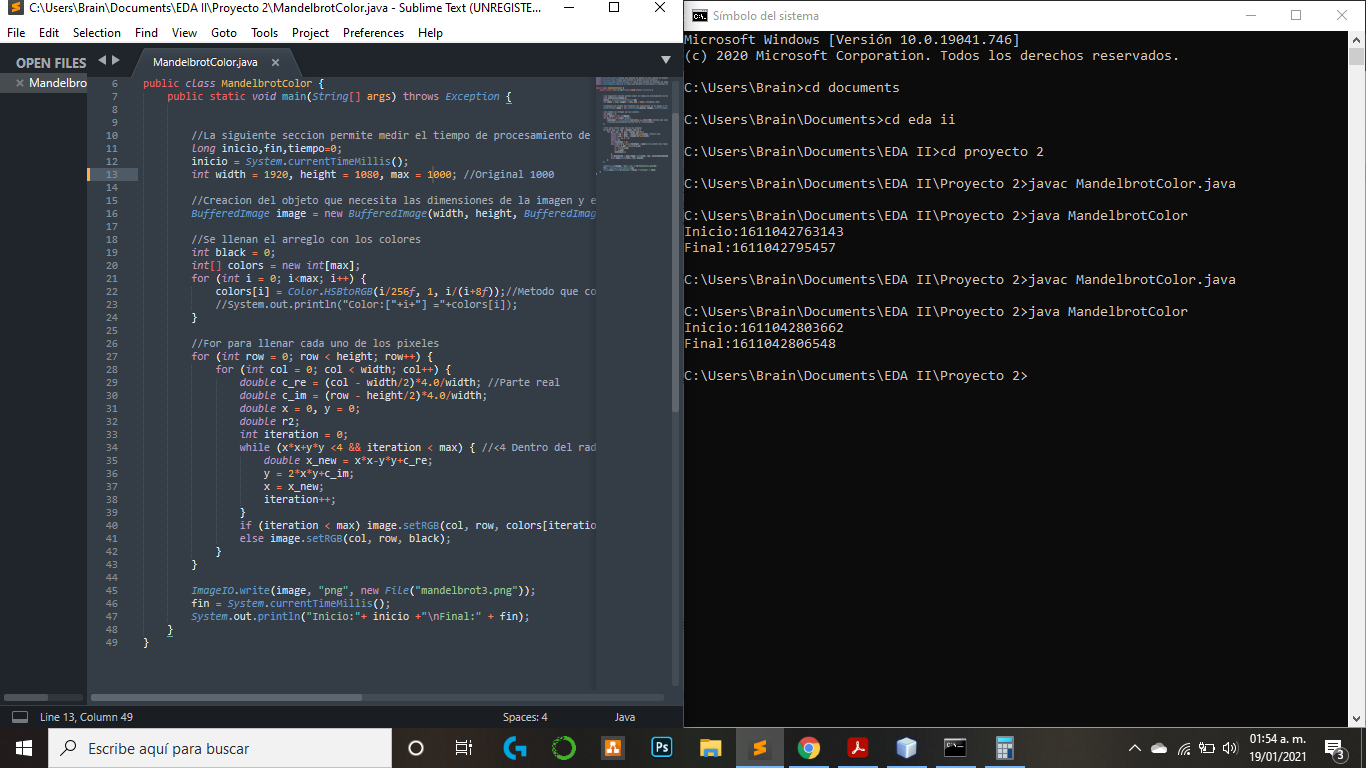
\includegraphics[scale=0.5]{secuencial}
				\caption{Prueba realizada, versión secuencial}
			\end{figure}
			\textbf{Tiempo de ejecución: 2886 ms.}
			
		\subsection{Pruebas para diferentes instancias}
		De acuerdo al programa, existen diversos parámetros con los cuales \textit{jugar} para crear imágenes tan diversas, pero manteniendo el conjunto de Mandelbrot.\\
		Entre estos parámetros encontramos algunos como el tamaño de la imagen (altura*anchura), el número de hilos para crear las imágenes, el número de imágenes que se crearán por cada hilo, la resolución inicial de nuestra primer imagen (con cuánto \textit{zoom} inicia), el aumento de resolución por imagen (el \textit{zoom} de una imagen a otra), la posición donde inicia la creación de las imágenes (pues se puede acercar a diversas áreas del conjunto de Mandelbrot), el número máximo de iteraciones (cuántas iteraciones deberán hacerse para comprobar si el punto diverge o no), o el color de la imagen.\\
		A continuación se muestran algunas de estas variaciones (todas involucradas en distintas imágenes), así como sus respectivos tiempos.\\
		
		\begin{figure}[!htb]
			\minipage{0.32\textwidth}
			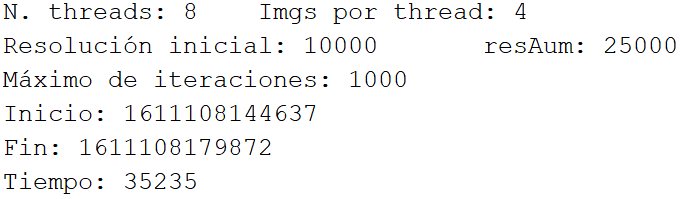
\includegraphics[width=\linewidth]{prueba2}
			\caption{Prueba 1}
			\endminipage\hfill
			\minipage{0.3\textwidth}
			
\includegraphics[width=\linewidth]{8threads_4pics_1}
			\caption{Imagen 1}
			\endminipage\hfill
			\minipage{0.3\textwidth}%
			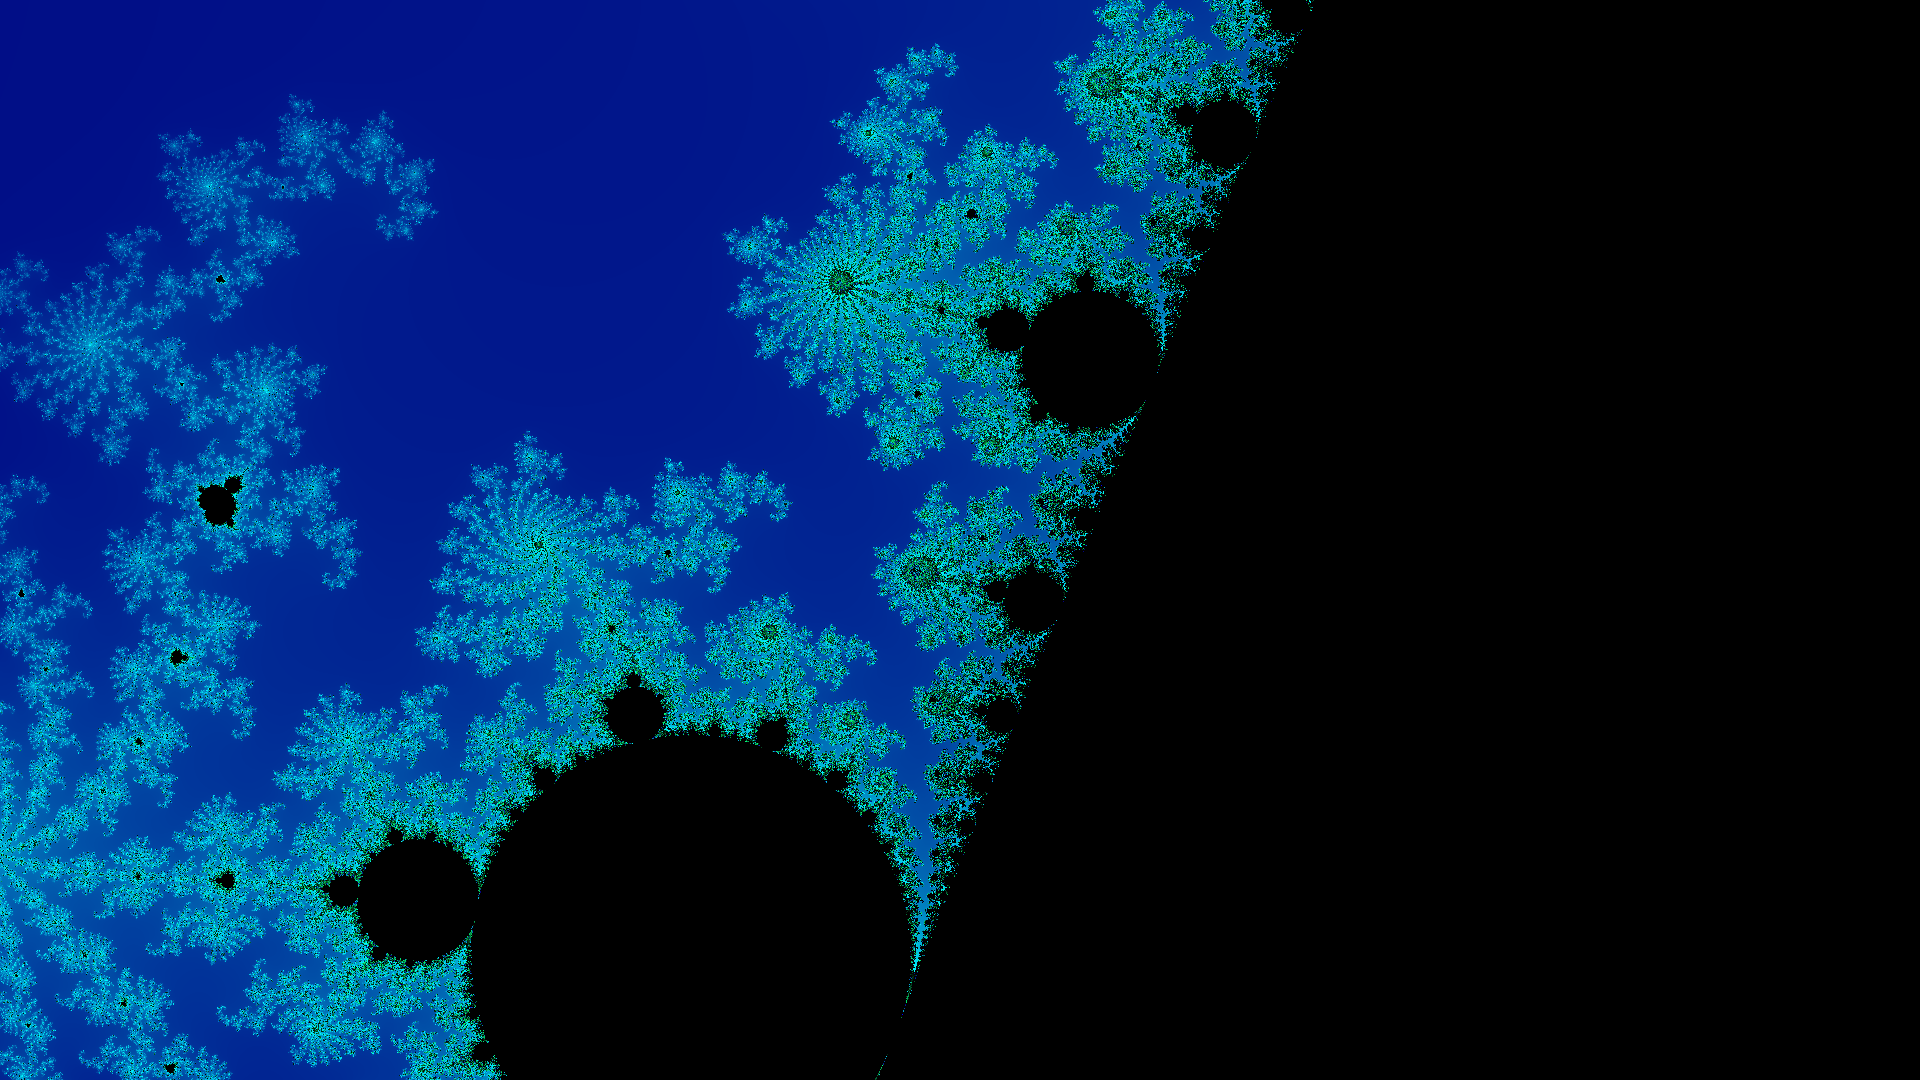
\includegraphics[width=\linewidth]{8threads_4pics_2}
			\caption{Imagen 2}
			\endminipage
		\end{figure}
		
		\begin{figure}[!htb]
			\minipage{0.32\textwidth}
			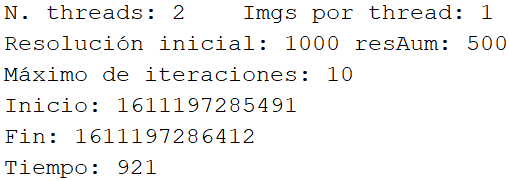
\includegraphics[width=\linewidth]{prueba2_10it}
			\caption{Prueba 2}
			\endminipage\hfill
			\minipage{0.3\textwidth}
			
\includegraphics[width=\linewidth]{2threads_1img_1}
			\caption{Imagen 1}
			\endminipage\hfill
			\minipage{0.3\textwidth}%
			
\includegraphics[width=\linewidth]{2threads_1img_2}
			\caption{Imagen 2}
			\endminipage
		\end{figure}
		
		\begin{figure}[!htb]
			\minipage{0.32\textwidth}
			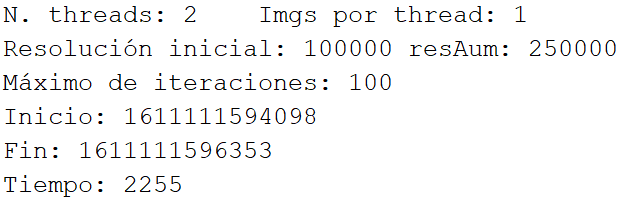
\includegraphics[width=\linewidth]{prueba_1threads_1pics4K_100it1_1}
			\caption{Prueba 3}
			\endminipage\hfill
			\minipage{0.3\textwidth}
			
\includegraphics[width=\linewidth]{1threads_1pics4K_100it1_1}
			\caption{Imagen 1}
			\endminipage\hfill
			\minipage{0.3\textwidth}%
			
\includegraphics[width=\linewidth]{1threads_1pics4K_100it1_2}
			\caption{Imagen 2}
			\endminipage
		\end{figure}
	
		\begin{figure}[!htb]
			\minipage{0.32\textwidth}
			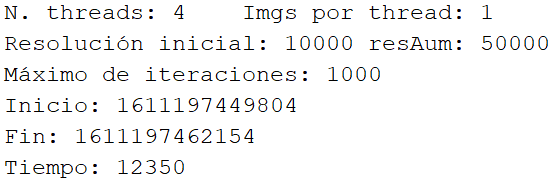
\includegraphics[width=\linewidth]{prueba4t_1img}
			\caption{Prueba 4}
			\endminipage\hfill
			\minipage{0.3\textwidth}
			
\includegraphics[width=\linewidth]{4threads_1img1}
			\caption{Imagen 1}
			\endminipage\hfill
			\minipage{0.3\textwidth}%
			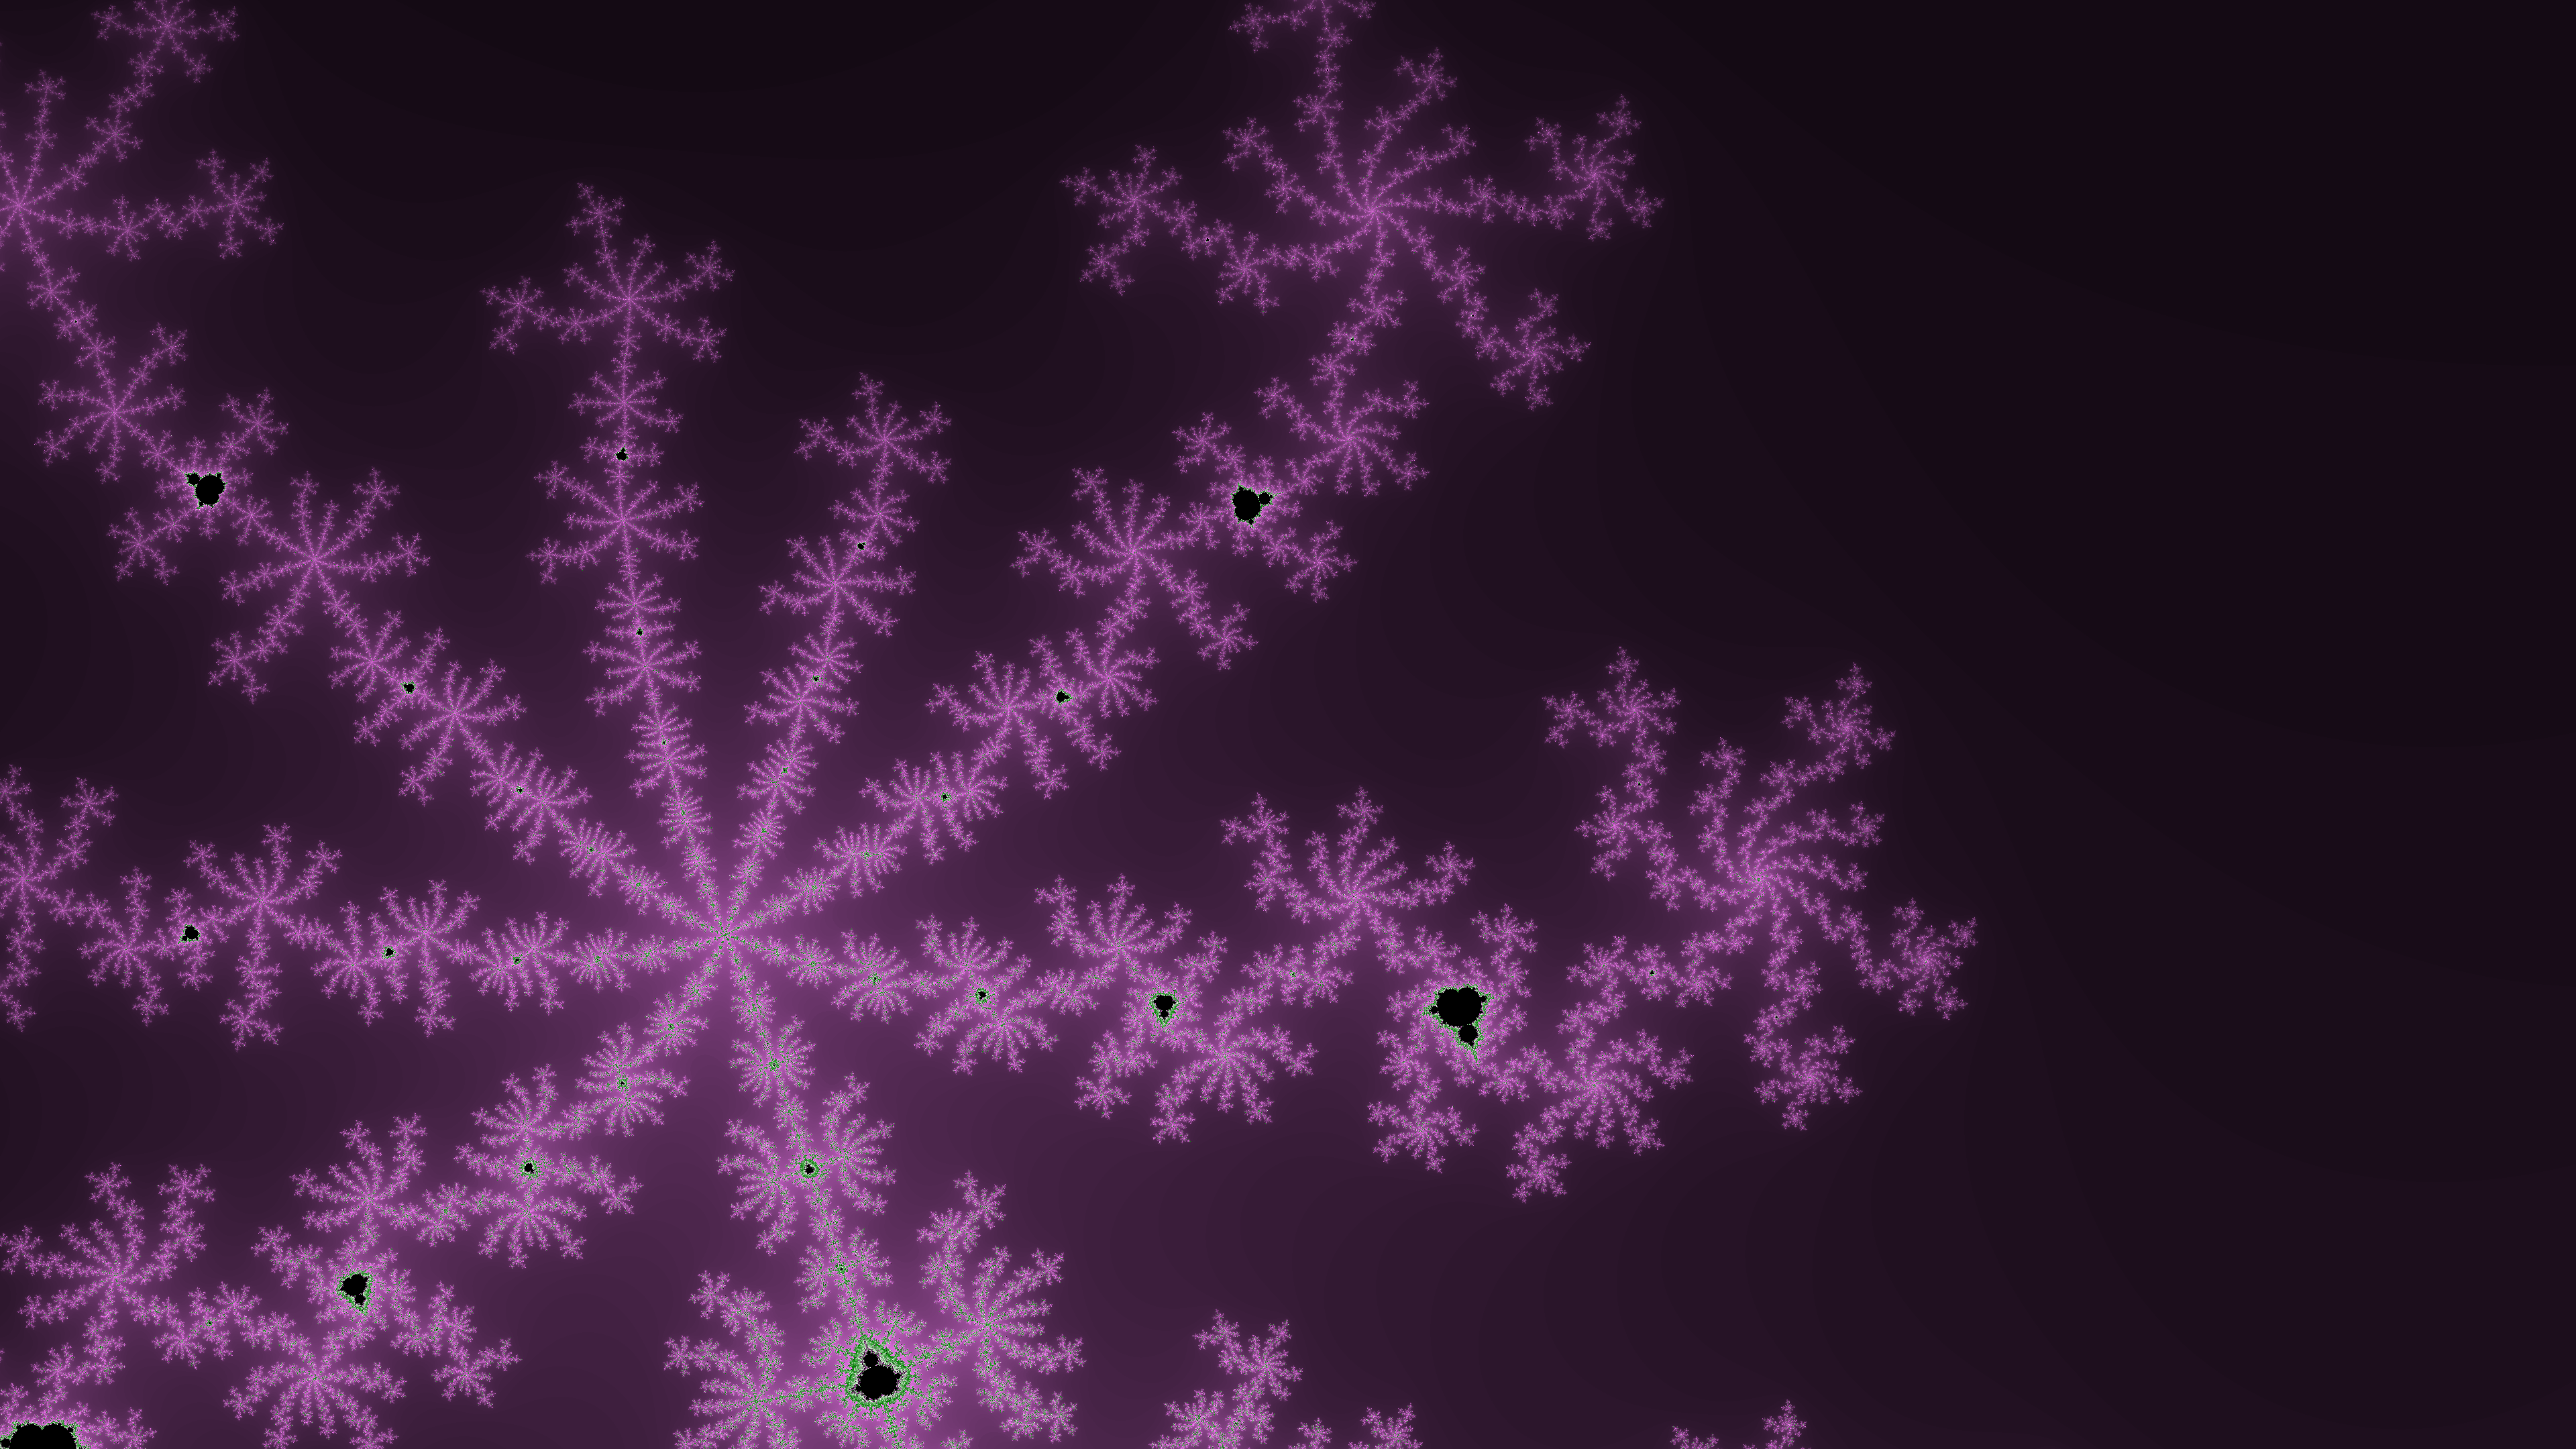
\includegraphics[width=\linewidth]{4threads_1img2}
			\caption{Imagen 2}
			\endminipage
		\end{figure}
	
		\begin{figure}[H]
			\minipage{0.32\textwidth}
			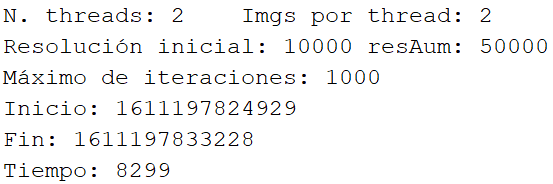
\includegraphics[width=\linewidth]{prueba2t_2img}
			\caption{Prueba 5}
			\endminipage\hfill
			\minipage{0.3\textwidth}
			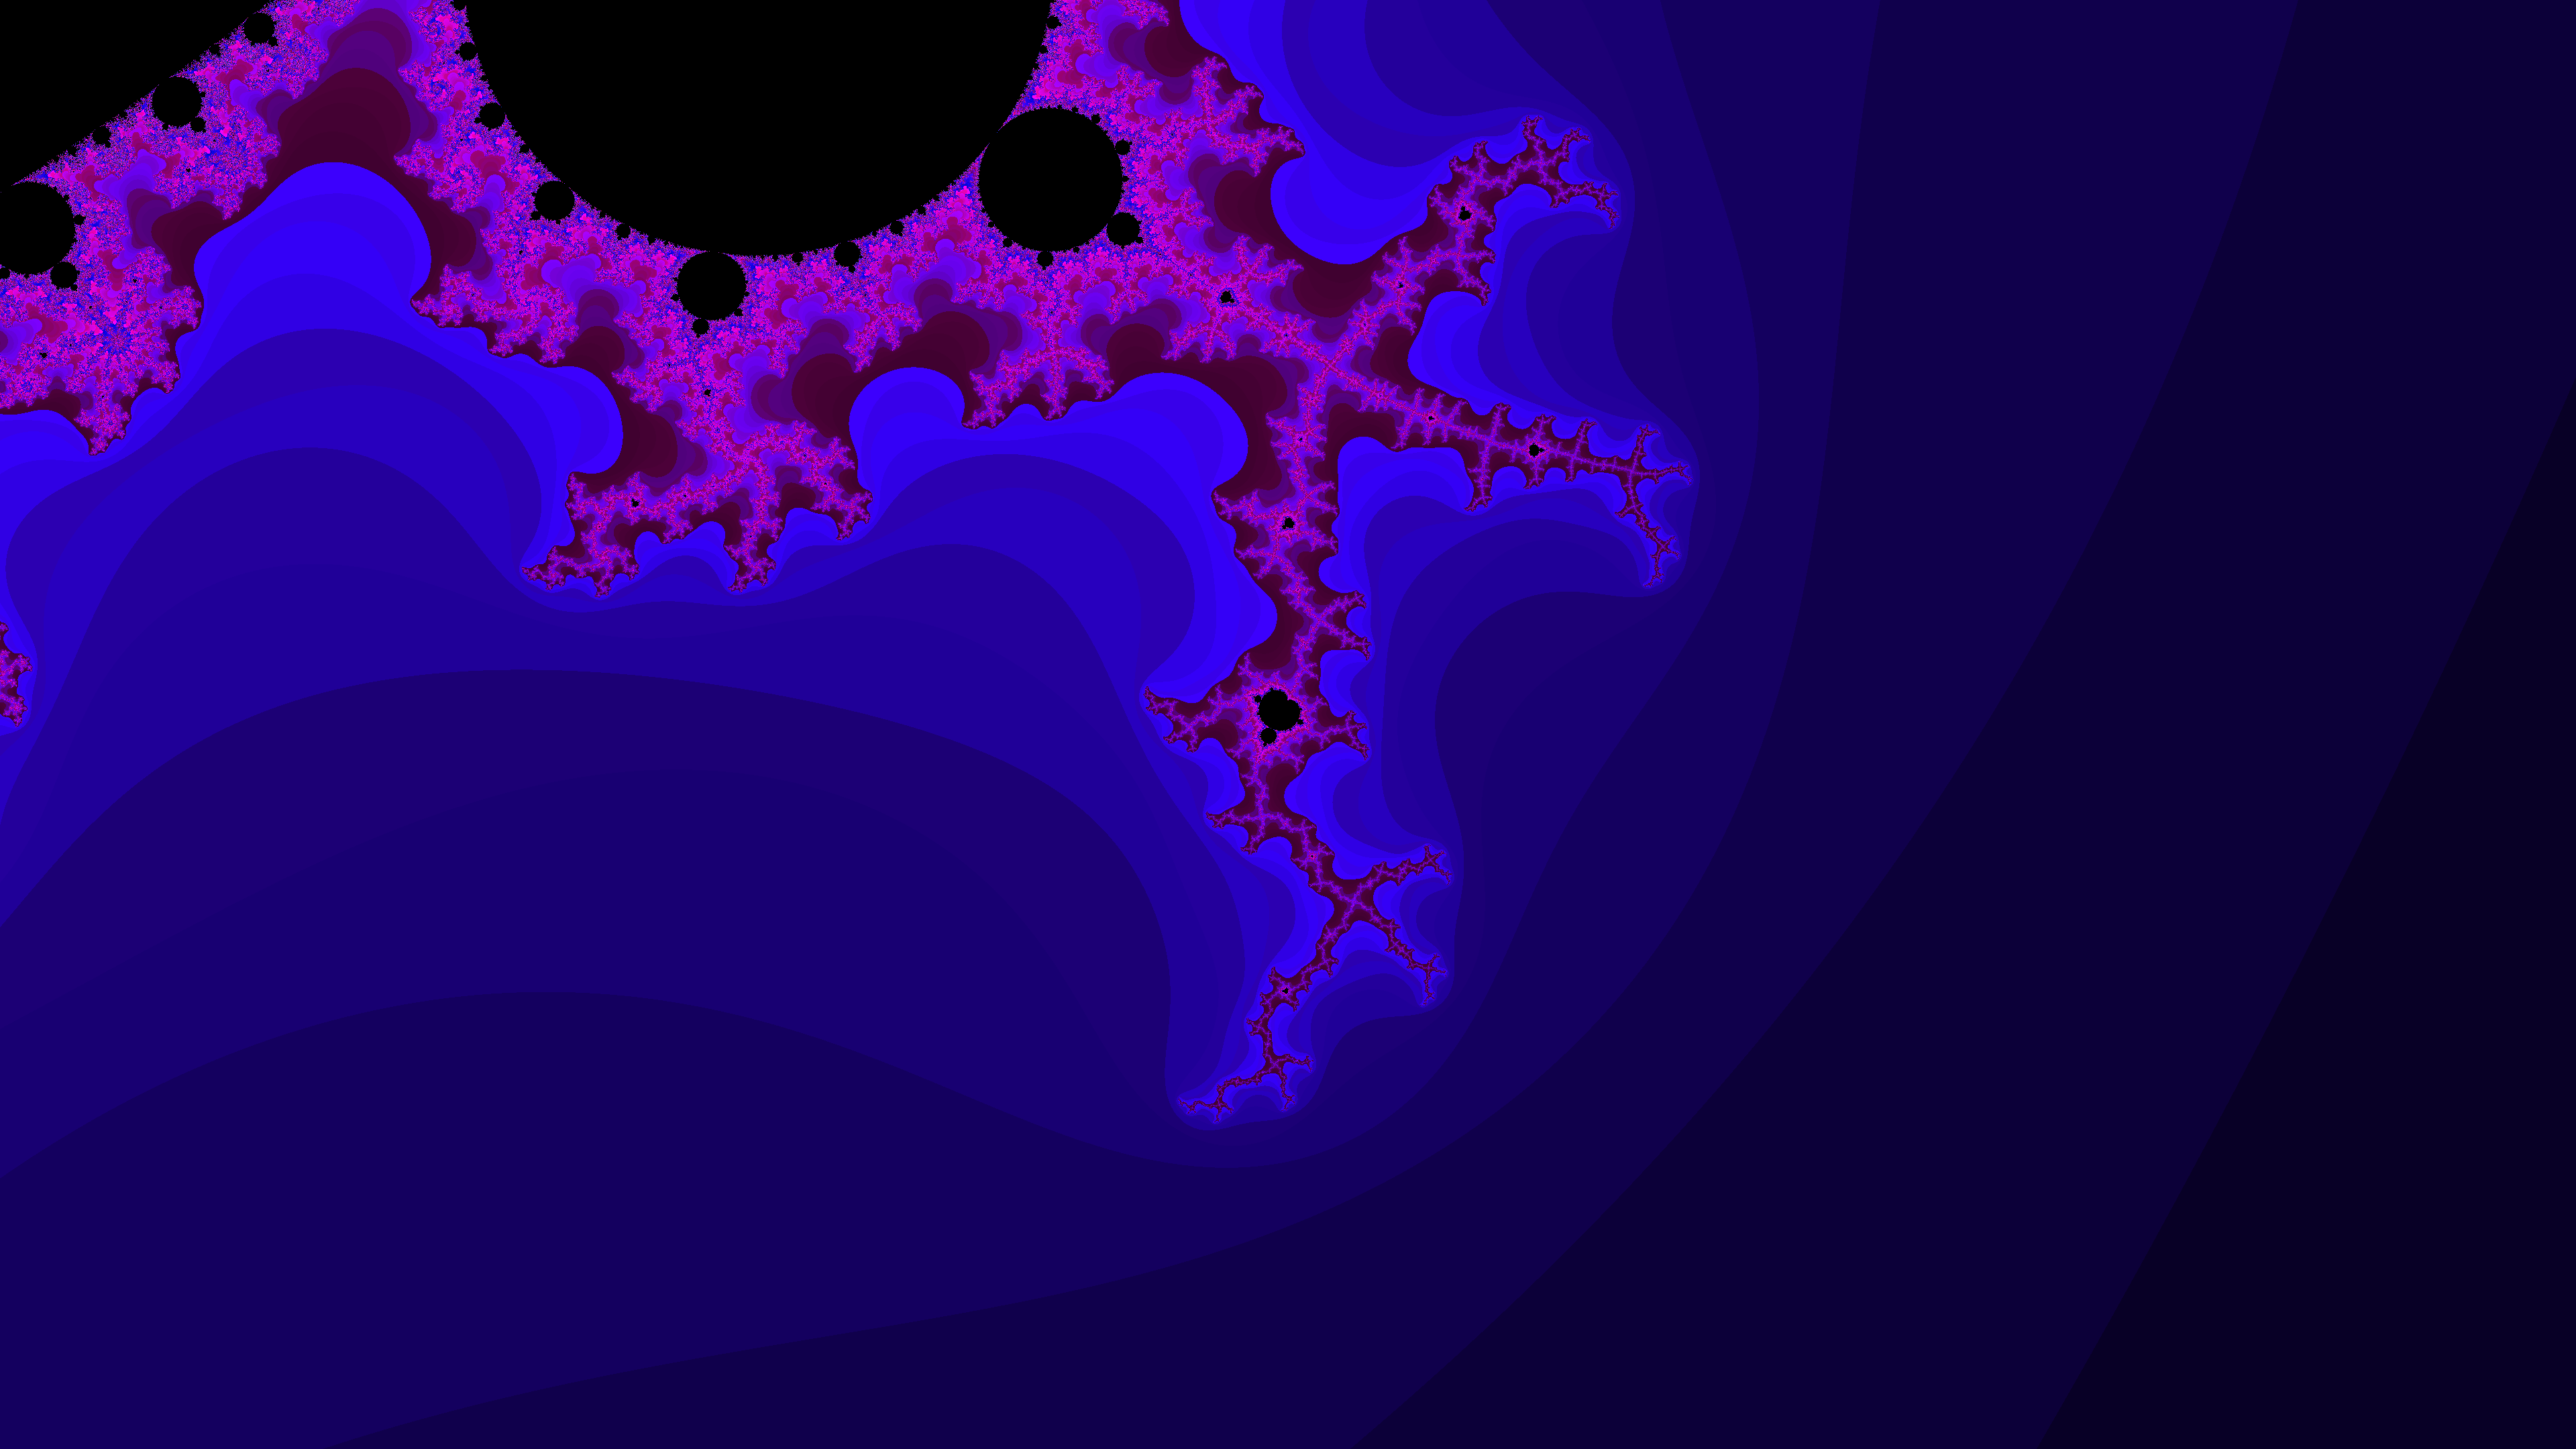
\includegraphics[width=\linewidth]{2threads_2img1}
			\caption{Imagen 1}
			\endminipage\hfill
			\minipage{0.3\textwidth}%
			
\includegraphics[width=\linewidth]{2threads_2img3}
			\caption{Imagen 2}
			\endminipage
		\end{figure}
		
		Podrían realizarse infinitas combinaciones con estos, y otros parámetros, para obtener imágenes tan alucinantes como las mostradas arriba. Con esto se demuestran diversas instancias y sus diversos resultados.
	
		\subsection{Gráficas}
		Se obtuvieron las siguientes gráficas a partir del tiempo de ejecución
		
		
			\begin{figure}[h]
				\centering
				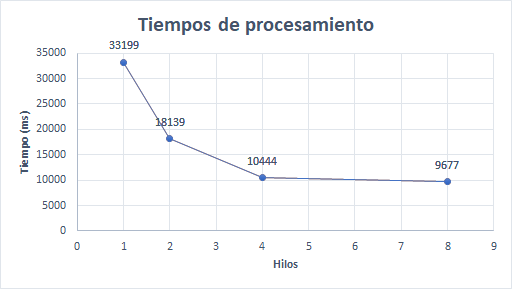
\includegraphics[scale=0.8]{Tiempos_de_procesamiento}
				\caption{Tiempos de procesamiento}
			\end{figure}
	
			\begin{figure}[H]
				\centering
				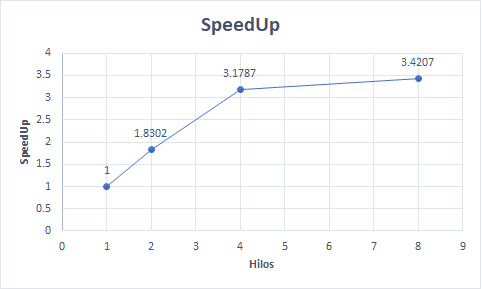
\includegraphics[scale=0.8]{SpeedUp}
				\caption{Speedup}
			\end{figure}
		
			\begin{figure}[H]
				\centering
				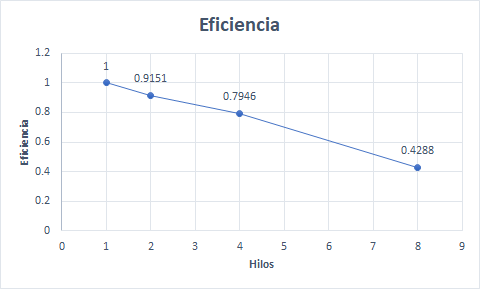
\includegraphics[scale=0.8]{Eficiencia}
				\caption{Eficiencia}
			\end{figure}
		
			\begin{figure}[H]
				\centering
				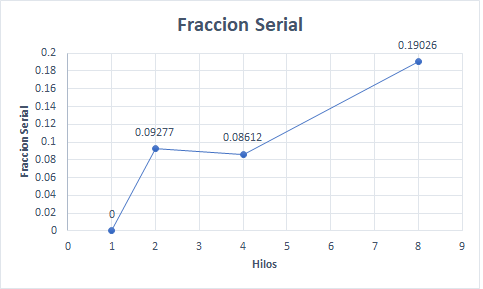
\includegraphics[scale=0.8]{Fraccion_serial}
				\caption{Fracción serial}
			\end{figure}
		
	
	\section{Conclusiones}
		\subsection{Díaz Hernández, Marcos Bryan}
			En la elaboración del proyecto fui aprendiendo poco a poco cómo el implementar los hilos en Java debido a que sí tengo la noción, pero para el caso de nuestro algoritmo, es necesario comprender el mismo paradigma y el lenguaje, por lo que en un determinado momento el paralelismo se tornó difícil de comprender por las distintas clases que se utiliza, pero analizando cada una de estas y la versión secuencial del algoritmo, me resultó mas fácil el poder comprender cómo se implementan los hilos, además de poder reconocer las características de un algoritmo paralelo, e incluso aprender algo nuevo sobre los fractales que fue sobre lo que se basó nuestro algoritmo. Debido a lo anterior considero que si se cumplió el objetivo que se planteo para el proyecto tanto el teórico como el de equipo. 
			
		\subsection{Lara Aguilar, Christian Abraham}
			Al realizar el proyecto ya tenía noción de qué eran los fractales y cómo se componían estos, pero algo que me sorprendió fue el cómo se coloreaban estos para dar lugar a aquellas imágenes que tiempo atrás me habían dejado anonadado debido a sus formas tan peculiares. Además de haber aprendido acerca de cómo se coloreaban, aprendí más, de acuerdo al objetivo general, los conceptos de la programación paralela a través de este algoritmo que elegimos, pues nos fue de gran utilidad el tener como algoritmo un fractal para poder asegurar, sin lugar a dudas, que el trabajo se realiza de una forma más práctica en cuanto a tiempos y recursos, desarrollándolo de una manera paralela que de la forma serial con la que hasta ahora se había trabajado en la carrera. Por último, creo que se cumplieron bien  los objetivos del equipo y los generales, pues también aprendí muchas cosas más acerca del uso propio de la creación de imágenes, el manejo de los hilos y la eficiencia de los programas paralelos.
			
	\section{Autoevaluación}
		
		Para el desarrollo de este problema tuvimos complicaciones con cierto integrante del equipo, por lo que nos fue más complicado desarrollar el proyecto entre dos personas, desconocemos las razones por las que decidió salir del equipo, pero igual comprendemos la presión de este fin de semestre. Pese a esto en nuestra humilde opinión creemos que hicimos un buen trabajo pues logramos repartirnos el trabajo para lograr cada punto solicitado, así como el programa paralelo y su versión secuencial. Además de esto, creemos que hicimos un buen trabajo resumiendo y explicando lo que implica el conjunto de Mandelbrot, pues se tiene que conocer acerca de ciertos aspectos matemáticos, expresiones, etc. También logramos crear varias imágenes, utilizando el programa paralelo, variando los parámetros para la creación de las mismas, por lo que considero eso es una prueba de que tenemos entendimiento del algoritmo y del código. Por estas implicaciones que se tuvieron al realizar el proyecto, así como lo que logramos realizar del proyecto, logrando cumplir nuestras expectativas finales, sentimos que sí realizamos un buen trabajo y logramos entender el paralelismo al nivel de comprensión de poder implementarlo en un algoritmo, así como haber entendido qué es el algoritmo que presentamos y todas las partes que lo conforman.
	
	\section{Referencias Bibliográficas}
		\begin{thebibliography}{3}
			\bibitem{latexcompanion} 
			Dejun Yan, et al. (2009). General Mandelbrot Sets and Julia Sets Generated from Non-analytic Complex Iteration. 17/01/2021. Dalian Nationalities University. Recuperado de: https://ieeexplore-ieee-org.pbidi.unam.mx:2443/stamp/stamp.jsp?tp=\&arnumber=5362044\&tag=1
			
			\bibitem{einstein} 
			Bhanuka Manesha. (2020). Efficient Generation of Mandelbrot Set using Message Passing Interface. 18/01/2021. Monash University Malaysia. Recuperado de: https://arxiv.org/pdf/2007.00745.pdf
			
			\bibitem{knuthwebsite} 
			Oracle. (2020). Java™ Platform, Standard Edition 8 API Specification. 16/01/2021, de Oracle. Recuperado de: https://docs.oracle.com/javase/8/docs/api/
		\end{thebibliography}
	
	
	
	
	
	
	
	
	
	
\end{document}